\section{代码块放置(Block Placement)}

\begin{frame}
    \frametitle{从CFG到代码布局(Code Layout) - Extended-TSP}

    控制流图(CFG)由若干基本块(Basic Blocks)组成,代码块放置的目标是让经常连在一起执行的基本块,在最终的代码布局(Code Layout)中放在一起,这样最直接的好处就是更好地利用 I-cache.

    事实上这个问题直到2021年才被形式化,背后的数学问题是 Ext-TSP \cite{mestre2021extended}. 给定无向图 $G = (V, E)$,带有正边权 $w: E \rightarrow R^{+}$,一个不递增的单调代价函数 $f(\cdot)$,满足 $f(1) = 1$,$f(i) = 0, i > k$,$k$是一个问题相关的常量.

    构建$V$的一个序列$d$,最优化

    \begin{equation}
        \sum_{(u, v) \in E} f(\left\lvert d_u - d_v \right\rvert) \cdot w(u, v)
    \end{equation}

    $d_u \in \lbrace 1, \dots, \left\lvert V \right\rvert \rbrace$,是$u$在序列中的位置.
\end{frame}

\begin{frame}
    \frametitle{控制流图链剖分 - Pettis-Hansen}

    首先对CFG建立链剖分,建立的原则是,经常被执行的边被放在一起,形成一条链(Chain).

    一条链包含一个或多个基本块(BB),并且每个路径都有一个优先级(priority)决定了他们在最终的代码布局中的情况.

    \begin{figure}
        \centering
        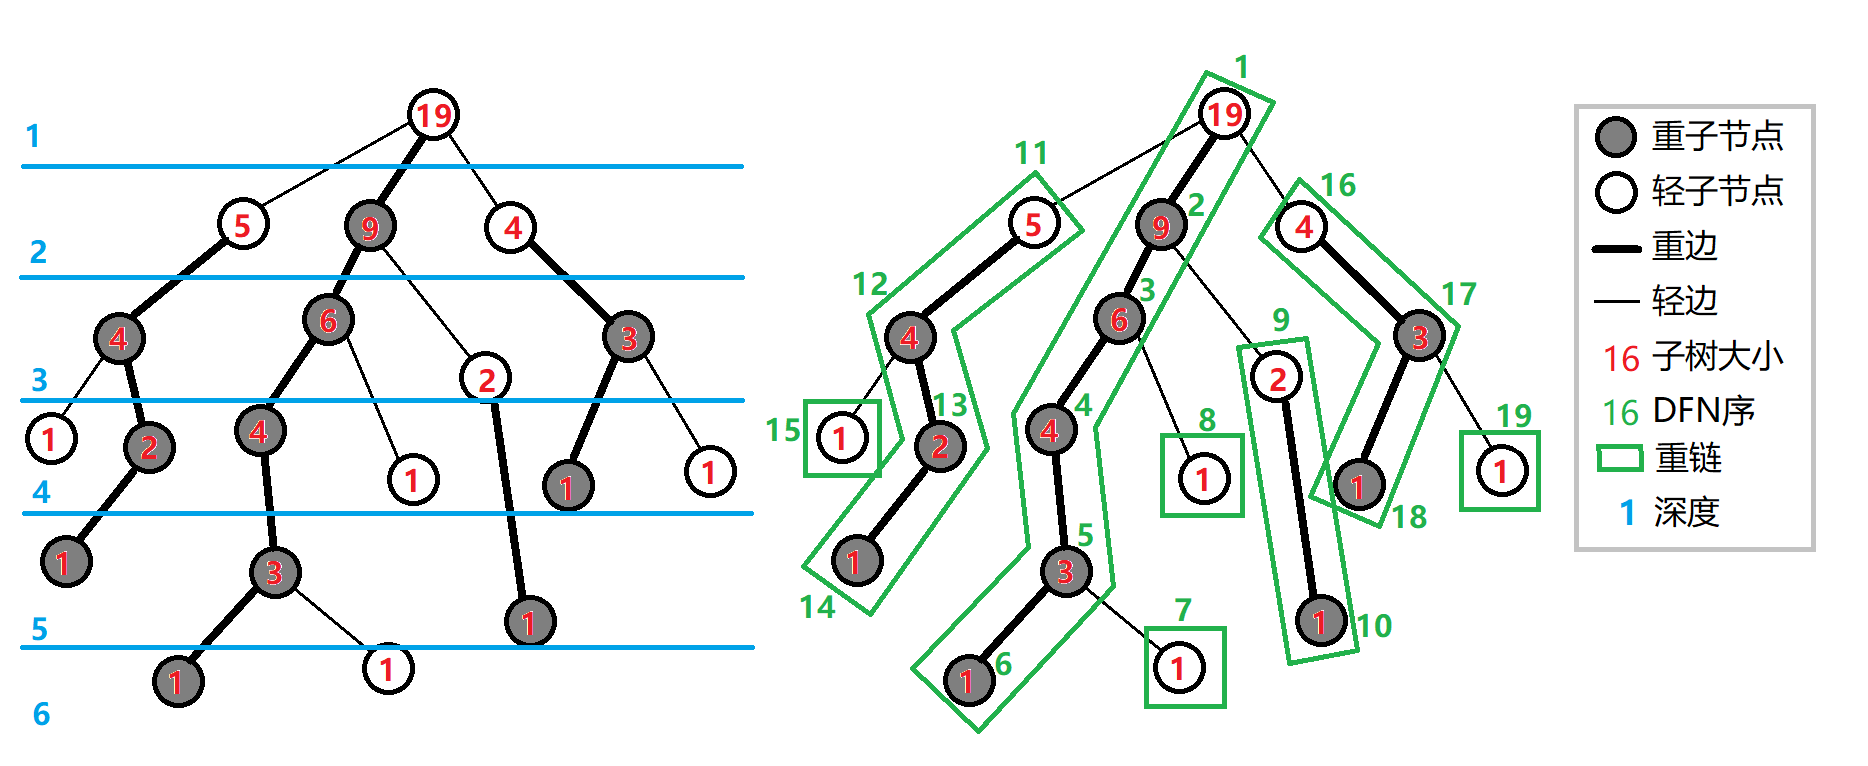
\includegraphics[width=0.64\textwidth]{images/hld.png}
        \caption{\cite{unknown-author-2022}轻重链剖分,树上链剖分的一种}
    \end{figure}

\end{frame}


\begin{frame}[fragile]
    \frametitle{Kruskal ? Prim ? - Pettis-Hansen}

    CFG没有树这么好的性质,CFG是一个有向图.构建链的方法是每次从边集合中选一条没有被选中的边(按照边的权重顺序),然后形成链状结构.

    \begin{figure}
        \centering
        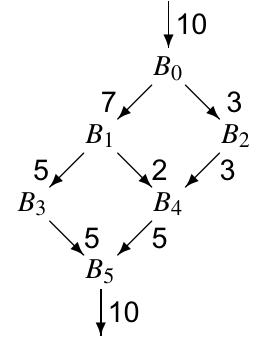
\includegraphics[width=0.24\textwidth]{images/example_cfg.png}
        \caption{CFG的一个例子\cite{cooper2011engineering}}
    \end{figure}



\end{frame}

\begin{frame}
    \frametitle{Greedy heuristic chain decomposition on CFGs}

    \begin{algorithmic}
        \State $E$ $\gets$ | edges |
        \For{each block b}
        \State make a degenerate chain, $d$, for $b$
        \State priority($d$) $\gets$ $E$
        \EndFor
        \State $P \gets 0$
        \For{each CFG edge $<x, y>, x \neq y$, in decreasing freq order}
        \State $ t \gets $ priority($a$)
        \State append $b$ onto $a$
        \State priority($a$) $\gets$ $\min$ ($t$, priority($b$), $P$++)
        \EndFor
    \end{algorithmic}


\end{frame}

\begin{frame}
    \frametitle{Greedy heuristic chain decomposition on CFGs}

    \begin{columns}
        \begin{column}{0.3\textwidth}
            \begin{figure}
                \centering
                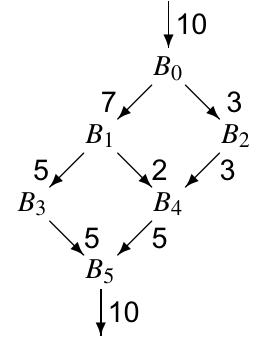
\includegraphics[width=0.8\textwidth]{images/example_cfg.png}
                \caption{CFG的一个例子\cite{cooper2011engineering}}
            \end{figure}
        \end{column}
        \begin{column}{0.6\textwidth}
            \begin{figure}
                \centering
                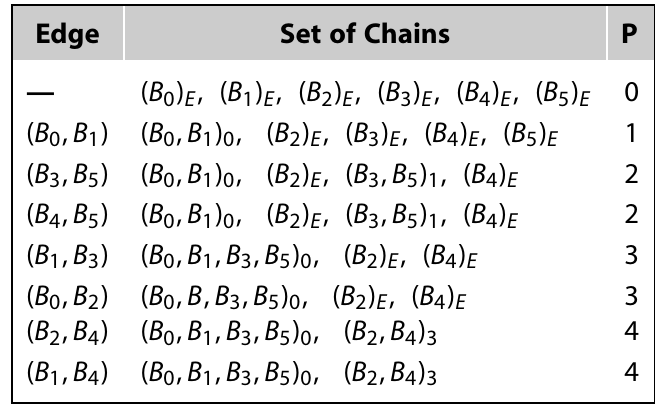
\includegraphics[width=0.8\textwidth]{images/greedy.png}
                \caption{算法每个过程选择的边,和对应的边集}
            \end{figure}
        \end{column}
    \end{columns}

\end{frame}


\begin{frame}
    \frametitle{基于WorkList组合最终的代码布局(Code Layout)}

    \begin{algorithmic}
        \State $t$ $\gets$ chain headed by the CFG entry node
        \State $WorkList$ $\gets$ $\lbrace(t, priority(t))\rbrace$ $ \qquad \Leftarrow$ Heap\cite{forsythe1964algorithms}
        \While{$WorkList \neq \emptyset$}
        \State remove a chian $c$ of lowest priority from $WorkList$
        \For{each block $x$ in $c$ in chain}
        \State place $x$ and the end of assembly codes
        \EndFor
        \For{each block $x$ in $c$}
        \For{each edge $<x, y>$ where $y$ is unplaced}
        \State $t \gets $ chain containing $<x, y>$
        \If{$(t, priority(t)) \notin WorkList$}
        $WorkList \gets WorkList \bigcup \lbrace (t, priority(t)) \rbrace$
        \EndIf
        \EndFor
        \EndFor
        \EndWhile
    \end{algorithmic}

\end{frame}


\begin{frame}
    \frametitle{Example}
    \begin{columns}
        \begin{column}{0.5\textwidth}
            \begin{figure}
                \centering
                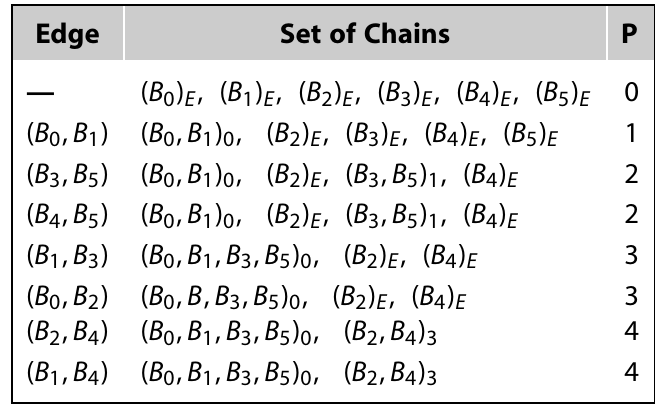
\includegraphics[width=0.86\textwidth]{images/greedy.png}
                \caption{上一个过程形成的链}
            \end{figure}
        \end{column}
        \begin{column}{0.5\textwidth}
            \begin{figure}
                \centering
                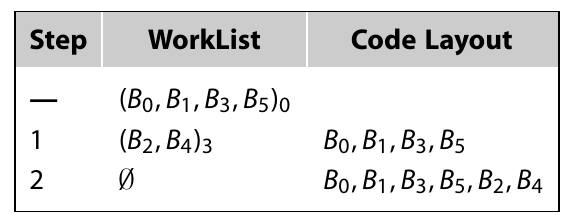
\includegraphics[width=0.78\textwidth]{images/worklist.png}
                \caption{生成最终的代码布局}
            \end{figure}
        \end{column}
    \end{columns}
\end{frame}